\section{Fourier Transform \tiny{(§13 (pp. 125-128), §15 (pp. 157-158), §19 (pp. 214-217), \cite{schilling2017measures})}}
We write \(L^1(\mathbb{R}^n)\) for \(L^1(\mathbb{R}^n, d\lambda_n)\).

The Fourier transform of a function \(f\in L^1(\mathbb{R}^n)\) is the function \(\hat{f}\) on \(\mathbb{R}^n\) defined by
\begin{align*}
    \hat{f}(x) = \frac{1}{(2\pi)^n} \int_{\mathbb{R}^n} f(y) e^{-i\langle x,y\rangle}dy,
\end{align*}w
where \(\langle x,y\rangle = x_1y_1 + ...+x_ny_n\). More generally, given a finite Borel measure \(\mu\), is \emph{Fourier transform} is the function \(\hat{\mu}\) on \(\mathbb{R}^n\) defined by
\begin{align*}
    \hat{\mu}(x) = \frac{1}{(2\pi)^n} \int_{\mathbb{R}^n} e^{-i\langle x,y\rangle}d\mu(y).
\end{align*}
We can also define \(\mu\) for complex Borel measures. 

\textbf{Warning.} There are many different conventions for the Fourier transform: instead of \(1/(2\pi^n)\) one also uses \(1, 1/(2\pi)^{u/2}\); instead of \(e^{-i\langle x,y\rangle }\) one also uses \(e^{i\langle x,y\rangle}, e^{\pm 2\pi i\langle x,y\rangle}\). 

Note that if \(\mu_f\) for \(f\in L^1(\mathbb{R}^n)\) is defined by \(d\mu_f=fd\lambda_n\), then 
\begin{align*}
    \hat{\mu}_f = \hat{f}.
\end{align*}

\begin{lemma}
    If \(\mu\) is a complex Borel measure on \(\mathbb{R}^n\), then \(\hat{\mu}\) is a Bounded continuous function on \(\mathbb{R}^n\), and \(|\hat{\mu}(x)|\leq \frac{|\mu|(\mathbb{R}^n)}{(2\pi)^n}\). 
\end{lemma}

In particular, if \(f\in L^1(\mathbb{R}^n)\), then \(\hat{f}\) is Bounded and continuous,
\begin{align*}
    |\hat{f}(x)|\leq \frac{||f||_1}{(2\pi)^n} \ \forall x.
\end{align*}
\ifdetailed 
\begin{proof}
    We have
\begin{align*}
    |\hat{\mu}(x)| &= \Big\vert \frac{1}{(2\hat{u})^n}\int_{\mathbb{R}^n}e^{-i\langle x,y\rangle}d\mu(y)\Big\vert \\
    &\leq \frac{1}{(2\hat{u})^n} \int_{\mathbb{R}^n}1d|\mu|(y) = \frac{1}{(2\hat{u})^n}|\mu|(\mathbb{R}^n).
\end{align*}
Continuity follows from the dominated convergence theorem.
\end{proof}
\fi
Some properties:
\begin{enumerate}[label=(\roman*)]
    \item If \(f_t(x) = f(x-t)\), then 
    \begin{align*}
        \hat{f}_t(y) = e^{-i\langle t,y\rangle}\hat{f}(y).
    \end{align*}
    \item If \(e_t(x) = e^{i\langle t,x\rangle}\), then
    \begin{align*}
        \hat{e_t f}(y) = \hat{f}(y-t).
    \end{align*} 
    \item If \(T\in GL_n(\mathbb{R})\) (invertible \(n\times n\) matrices), then
    \begin{align*}
        \hat{f\circ T} = |\det T|^{-1}\hat{f}\circ(T^t)^{-1}.
    \end{align*}
    \ifdetailed
    \begin{proof}
        \begin{align*}
            \hat{f\circ T}(x) &= \frac{1}{(2\pi)^n} \int_{\mathbb{R}^n} f(Ty)e^{-i\langle x,y\rangle} dy \\
            &= \frac{1}{|\det T|}\frac{1}{(2\pi)^n} \int_{\mathbb{R}^n} f(y)e^{-i\langle x,T^{-1}y\rangle} dy\\
            &= \frac{1}{|\det T|}\frac{1}{(2\pi)^n} \int_{\mathbb{R}^n} f(y)e^{-i\langle (T^t)^{-1}x,y\rangle} dy \\
            &= \frac{1}{|\det T|}\hat{f}((T^t)^{-1}x).
        \end{align*}
    \end{proof}
    \fi 
    \item \(\hat{\bar{f}}(x) = \bar{\hat{f}}(-x)\).
\end{enumerate}
\textbf{Important example.} 

If \(f(x) = e^{-\frac{|x|^2}{2}}\) (\(|x|=\langle x,x\rangle^{1/2}\)), then \(\hat{f}(x) = 1/(2\pi)^n e^{-\frac{|x|^2}{2}}\).
\ifdetailed
\begin{proof}
    We need to show that 
    \begin{align*}
        \frac{1}{2\pi}\int_{\mathbb{R}^n} e^{-\frac{y^2}{2}-ixy}dy = \frac{e^{-\frac{x^2}{2}}}{(2\pi)^{1/2}}.
    \end{align*}
    We have \(e^{-\frac{y^2}{2}-ixy} = e^{-\frac{1}{2}(y+ix)^2-\frac{x^2}{2}}\), so we need to check that
    \begin{align*}
        \frac{1}{\sqrt{2\pi}} \int_{\mathbb{R}}e^{-\frac{1}{2}(y+ix)^2}dy = 1
    \end{align*}
    \begin{figure}[H]
        \centering
        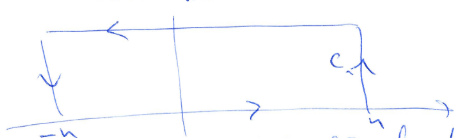
\includegraphics[scale=0.5]{Figs/for_proof_fourieridentity.png}
    \end{figure}
    Let \(c_n\) be as in the figure above, and consider \(\oint e^{-\frac{z^2}{2}}dz = 0\). Letting \(n\rightarrow\infty \), we concolude that 
    \begin{align*}
        \int_{\mathbb{R}^n}e^{-\frac{1}{2}(y+ix)^2}dy = \int_{\mathbb{R}^n} e^{-\frac{y^2}{2}}dy.
    \end{align*}
    It remains to show that 
    \begin{align*}
        \frac{1}{\sqrt{2\pi}}\int_{\mathbb{R}} e^{-\frac{y^2}{2}}dy = 1.
    \end{align*}
    Let \(a= \int_{0}^{\infty}e^{-\frac{y^2}{2}}dy\), so \(\int_{\mathbb{R}} e^{-\frac{y^2}{2}}dy = 2a\). Then \(a^2 = \int_{0}^{\infty}\int_{0}^{\infty}e^{-\frac{x^2+y^2}{2}}dxdy\). Passing to spherical coordinates we get \(a^2= \int_{0}^{\infty}dr\int_{0}^{\frac{\pi}{2 }}d\phi e^{-\frac{r^2}{2}}r = \frac{\pi}{2}\int_{0}^{\infty}dr e^{-\frac{r^2}{2}}r = \frac{\pi}{2}\). Therefore \(2a = \sqrt{2\pi}\).
\end{proof}
\fi 
More generally, if \(f(x) = e^{-\frac{c|x|^2}{2}}\), then 
\begin{align*}
    \hat{f}(x) = \frac{1}{(2\pi c)^{\frac{u}{2}}} e^{-\frac{|x|^2}{2c}} \ \forall c>0.
\end{align*}
This follows from property (iii).

For functions \(f,g\) on \(\mathbb{R}^n\), their \textbf{convolution} is the function \(f\times g\) defined by
\begin{align*}
    (f\ast g)(x) \eqdef \int_{\mathbb{R}^n} f(y) g(x-y) dy = \int_{\mathbb{R}^n} f(x-y)g(y) dy
\end{align*}
when is this well-defined?
\begin{lemma}
    If \(f,g\in L^1(\mathbb{R}^n)\), then the function \(y\mapsto f(y)g(x-y)\) is integrable for \((\lambda_n)\)-a.e. \(x\), \(f\ast g\in L^1(\mathbb{R}^n)\) and \(||f\ast g||_1\leq||f||_1 ||g||_1\).
\end{lemma}
\ifdetailed 
\begin{proof}
    For everything except the last inequality we may assume that \(f,g\geq 0\). Consider \(F:\mathbb{R}^n\times\mathbb{R}^n\rightarrow [0,\infty)\),
    \begin{align*}
        F(x,y) = f(x-y)g(y).
    \end{align*}
    Then 
    \begin{align*}
        \int_{\mathbb{R}^n}\left(\int_{\mathbb{R}^n}F(x,y)dx\right)dy &= \int_{\mathbb{R}^n}\left(\int_{\mathbb{R}^n}f(x-y)dx\right)g(y)dy \\
        &=||f||_1\int_{\mathbb{R}}g(y)dy = ||f||_1 ||g||_1. 
    \end{align*}
    Therefore, by Tonelli's theorem, \(F\in L^1(\mathbb{R}^n\times\mathbb{R}^n)\). Then, by the same theorem, 
    \begin{align*}
        ||F||_1 = \int_{\mathbb{R}^n}\left(\int_{\mathbb{R}^n}F(x,y)dy\right)dx = \int_{\mathbb{R}^n}\left(\int_{\mathbb{R}^n}f(y)g(x-y)dy\right)dx.
    \end{align*}
    It follows that \(\int_{\mathbb{R}}f(y)g(x-y)dy<\infty\) for a.e. \(x\), the function 
    \begin{align*}
        x\mapsto (f\ast g)(x) = \int_{\mathbb{R}^n}F(x,y) dy
    \end{align*}
    is measurable and \(||f\ast g||_1 = ||F||_1 = ||f||_1 ||g||_1\). 

    Finally, for general \(f,g\in L^1(\mathbb{R}^n)\), 
    \begin{align*}
        ||f\ast g||_1 &= \int_{\mathbb{R}^n}\Big\vert \int_{\mathbb{R}^n}f(y)g(x-y)dy\Big\vert dx \\
        &\leq \int_{\mathbb{R}^n}\left(\int_{\mathbb{R}^n} |f(y)|\cdot |g(x-y)|dy\right)dx \\ 
        &= || |f|\ast |g|||_1 = |||f|||_1 \cdot || |g| ||_1 = ||f||_1\cdot ||g||_1.
    \end{align*}
\end{proof}
\fi 

Next let us show that \(f\ast g\) is well-defined for \(f\in L^1(\mathbb{R}^n)\), \(g\in L^p(\mathbb{R}^n)\), \(1\leq p \leq \infty\).

\begin{lemma}
    Assume \(\phi:(a,b)\rightarrow \mathbb{R}\) is a convex function. Then \(\phi\) is continuous and \(\phi(x) = \sup\{ l(x):\phi\geq l, l(s)=\alpha s+\beta \}\).
\end{lemma}
\ifdetailed
\begin{proof}
    We clamin that the function \(t\mapsto \frac{\phi(t)-\phi(x)}{t-x}\), \(t\neq x\), is increasing for all \(x\). This is equivalent to the inequalities:
    \begin{align*}
        \frac{\phi(t)-\phi(x)}{t-x} \leq \frac{\phi(y)-\phi(x)}{y-x}\leq \frac{\phi(y)-\phi(t)}{y-t},
    \end{align*}
    for \(a<x<t<y<b\). To prove the inequalities write \(t=\lambda x + (1-\lambda)y\), \(0<\lambda<1\). Then
    \begin{align*}
        \frac{\phi(t)-\phi(x)}{t-x} &\leq \frac{\lambda \phi(x) + (1-\lambda)\phi(y) - \phi(x)}{t-x} = \frac{\phi(y)-\phi(x)}{y-x}, \\
        \frac{\phi(y)-\phi(t)}{y-t} &\geq \frac{\phi(y) -\lambda\phi(x) - (1-\lambda)\phi(y)}{y-t} = \frac{\phi(y)-\phi(x)}{y-x},
    \end{align*}
    prooving the claim. 

    The claim implies that the left and right derivatives \(\phi'_{-}\) and \(\phi'_{+}\) exist and
    \begin{align*}
        \frac{\phi(t_1)-\phi(x)}{t_1-x} \leq \phi'_{-}(x)\leq \phi'_{+}(x) \leq \frac{\phi(t_2) -\phi(x)}{t_2 - x},
    \end{align*}    
    for \(t_1<x<t_2\). From the existence of \(\phi'_{-},\phi'_{+}\) we conclude that \(\phi\) is continuous. We see also that for \(l(s)=\phi'_{+}(x)(s-x) + \phi(x)\) we have \(\phi\geq l\) and \(\phi(x) = l(x)\).
\end{proof}
\fi 
\begin{theorem}[Jensen's inequality]
    Assume \((X,\mathscr{B}, \mu)\) is a probability measure space (so \(\mu(x)=1\)), \(\phi:[0,\infty) \rightarrow [0,\infty)\) is a convex function. Then, for every integrable function \(f:X\rightarrow[0,\infty)\) we have 
    \begin{align*}
        \phi\left(\int_X fd\mu\right) \leq \int_X \phi\circ f d\mu.
    \end{align*}
    The same inequality holds for any measurable \(f:X\rightarrow [0,\infty]\) if \(\lim_{x\rightarrow\infty}\phi(x) = +\infty \) and we put \(\phi(+\infty) = +\infty\).
\end{theorem}
\ifdetailed 
\begin{proof}
    Note that as \(\phi\) is continuous on \((0,\infty)\) the function \(\phi\circ f\) is measurable. If \(\int_X fd\mu=0\), so \(f=0\) a.e., then there is nothing to prove, as then
    \begin{align*}
        \phi\left(\int_X fd\mu\right) = \phi(0), \ \int_X \phi\circ fd\mu = \phi(0)\mu(X) = \phi(0).
    \end{align*}
    Assume therefore that \(f:X\rightarrow[0,\infty)\) and \(t=\int_X fd\mu\) satisfies \(0<t<\infty\). Take a linear function \(l(s) = \alpha s + \beta\) s.t. \(\phi\geq l\) on \((0,\infty)\). Then also \(\phi(0)\geq l(0)=\beta\). (Indeed, for \(s>0\) we have \(l(s) \leq \phi(s) \leq (1-s)\phi(0) + s\phi(1)\), and letting \(s\downarrow 0\) we get \(\phi(0)\geq \l(0)\).) Then 
    \begin{align*}
        l\left(\int_X fd\mu\right) &= \alpha \int_X fd\mu + \beta \\
        &=\int_X l\circ fd\mu \leq \int_X \phi\circ fd\mu.
    \end{align*}
    Taking the supremum over \(l\) as above, by the previous lemma, we get 
    \begin{align*}
        \phi\left(\int_X fd\mu\right) \leq \int_X \phi\circ fd\mu.
    \end{align*}
    Assume now that \(\lim_{x\rightarrow\infty}\phi(x) = \infty\) and put \(\phi(\infty) = \infty\). 

    If \(f:X\rightarrow [0,\infty]\) and \(\int_X fd\mu<\infty\) (so \(f<\infty\) a.e.), then the same proof as above gives the required inequality. It remains to show that if 
    \begin{align*}
        \int_X fd\mu = \infty, \text{ then also } \int_X \phi\circ fd\mu=\infty.
    \end{align*}
    For this it suffices to show that there is \(l(s)=\alpha s + \beta\) s.t. \(\phi\geq l\) and \(\alpha>0\), as then 
    \begin{align*}
        \int_X \phi\circ fd\mu \geq \alpha\int_X fd\mu + \beta = \infty.
    \end{align*}
    Such and \(l\) exists by the proof of the previous lemma: take \(t>0\) and find \(x\) s.t. \(\phi(x) >\phi(t)\). Then 
    \begin{align*}
        \phi'_{+}(x) \geq \frac{\phi(t) - \phi(x)}{t-x}>0 
    \end{align*}
    and we can take \(l(s) = \phi'_{+} (x) (s-x) + \phi(x)\).
\end{proof}
\fi 